\documentclass[a4paper,12pt]{report}
\usepackage[utf8]{inputenc}
\usepackage{amsmath}
\usepackage{graphicx}
\usepackage{listings}
\usepackage{tikz}
\usepackage[T1]{fontenc}
\usepackage{color}
\usetikzlibrary{arrows,automata}
\definecolor{pythonred}{rgb}{0.6,0,0} % for strings
\definecolor{pythongreen}{rgb}{0.25,0.5,0.35} % comments
\definecolor{pythonpurple}{rgb}{0.5,0,0.35} % keywords
	\definecolor{pythondocblue}{rgb}{0.25,0.35,0.75} % javadoc
	 
	\lstset{language=python,
	basicstyle=\ttfamily,
	keywordstyle=\color{pythonpurple}\bfseries,
	stringstyle=\color{pythonred},
	commentstyle=\color{pythongreen},
	morecomment=[s][\color{pythondocblue}]{/**}{*/},
	numbers=left,
	numberstyle=\tiny\color{black},
        stepnumber=2,
	numbersep=10pt,
	tabsize=4,
	showspaces=false,
	showstringspaces=false}

% Title Page

 \title{\bfseries\huge \textcolor{purple}{\underline {Software Lab}} \\{\textcolor{blue}{Assignment3 :Design Weather Forecasting App In Tcl/tk}}}
\author{\bfseries\large\textcolor{black}  {Harshit Kumar Gupta}\\ {\textcolor{black} {2013EET2369 }}\\

\includegraphics[width=3cm,height=3.4cm]{./iit.png}\\\noindent Computer Technology\\
\noindent Department Of Electrical Engineering\\IIT DELHI}
% iit.png: 282x282 pixel, 72dpi, 9.95x9.95 cm, bb=0 0 282 282
\begin{document}
\maketitle
\tableofcontents


\chapter{\textcolor{blue}{\underline {PROBLEM STATEMENT}}}
\noindent Develop an ubuntu app which can accomplish following two tasks:
\begin{enumerate}
 \item  forecasting next few days weather conditions
 \item   keep record of past few days' weather conditions (max 30 days) in to your database and show it as a strip chart which has a rewind / fast fwd button.
\end{enumerate}

\noindent Use tcl/tk for the GUI to interact with the user and scripting languages like python,perl,shell,awk etc  for other operations. The user will be asked to enter name of a place for  which weather conditions have to be forecasted, the number of days (n) for which to show information, and to press a button to decide whether to forecast or tell about the past n days' weather conditions.\\\\
For keeping the record of past few days' weather information, you can use MySQL database. Max 5 days' information need to be recorded.
You can make use of yahoo api for weather forecasting info. It easily tells about the next five days' weather conditions.
Develop html webpage using Doxygen to publicize your app.\\\\


\begin{center}
\chapter{\textcolor{blue}{\underline {ABSTRACT}}}
\end{center}
\noindent The intention is to teach how to design the User Interface in your programming assignment. Though it is the most important part of the user interaction, and the most likely to draw adverse comment, it is also the most neglected part of coding. May be because engineers do not understand a good interface intuitively. A good interface design can be taught, developing a great interface is an art to be developed by systematic application of processes and is difficult to master.

There are many tools which allow a basic UI to be cobbled together. For example, tcl/tk (and the wish shell) was developed by John Ousterhout to allow quick interfaces and shells to be thrown together. 4GL (4th Generation Languages) such as RAD tools (Delphi), IDEs such as Athena make this process easy and a lot less scary. In Ubuntu, try Anjuta or Glade or Fox/GLUT. In Windows, VisualStudio does an effective job of UI design.
\begin{center}
\chapter{\textcolor{blue}{\underline {INTRODUCTION}}}
\end{center}
\noindent Tcl is a string-based command lan- guage. The language has only a few fundamental constructs and relatively little
syntax, which makes it easy to learn. The Tcl syntax is meant to be simple. Tcl is designed to be a glue that assembles software building blocks into applications.
A simpler glue makes the job easier. In addition, Tcl is interpreted when the application runs. The interpreter makes it easy to build and refine your applica-
tion in an interactive manner.\\\\
MySQL  also called "My Sequel" is the world's second most widely used open-source relational database management system (RDBMS). The SQL phrase stands for Structured Query Language.
The MySQL development project has made its source code available under the terms of the GNU General Public License, as well as under a variety of proprietary agreements. MySQL was owned and sponsored by a single for-profit firm, the Swedish company MySQL AB, now owned by Oracle Corporation.\\

MySQL is a popular choice of database for use in web applications, and is a central component of the widely used LAMP open source web application software stack (and other 'AMP' stacks). LAMP is an acronym for "Linux, Apache, MySQL, Perl/PHP/Python." Free-software-open source projects that require a full-featured database management system often use MySQL.

\begin{center}
\chapter{\textcolor{blue}{\underline {SPECIFICATIONS AND ASSUMPTIONS}}}
\end{center}
\section*{Specifications}

\begin{enumerate}
\item Tcl/tk script is used to create the GUI for the User.
\item 'wget' Command is used to generate the xml file which contains the weather information of the city.
\item Doxygen has been used for proper Documentation.
\item For various uses Bash has also been used accordingly.
\item Yahoo API has beenn used for Weather Predictions.
\item The Temperature calculated comes out to be in Celsius.

\end{enumerate}

\section*{Assumptions}

\begin{enumerate}
\item The User is required to Input a valid city name.
\item Weather Forecasting Includes date, day , low and high Temperature.
\item The SQL Server table values may not have a primary key attribute as specifically not required.
\item Data may be only used for Information and not Commercial Purpose.
\end{enumerate}
 
\begin{center}
\chapter{\textcolor{blue}{\underline {LOGIC USED/METHODOLOGY}}}
\end{center}
The methodology that is used for developing the program is defined below:\\

\begin{enumerate}
\item Basically , We intiate our code in tcl script to create a User Interface.
\item Now as the User is required to input the value into the text box which is a city name.
\item We make the use of Yahoo ApI to get the value of the woeid(where on earth id)
\item This woeid value generated is passed to the Yahoo Developer Url which geographically calculates the weather Conditions
\item This Weather Conditions are detailed in a XML file which are further Parsed into the tcl Script.
\item Now the values parsed are Stored into the SQL database Table using mysql.
\item Finally the entry values of this table are taken bby the tcl script.
\item The present Weather Conditions and for the next 5 days are displayed using the GUI.
\item Past few values for the weather Predictions are stored in the DB and can be fetched as required.
\end{enumerate}

\begin{center}
\chapter{\textcolor{blue}{\underline {FLOWCHART}}}
\end{center}
\noindent \\Flowchart
\begin{center}
 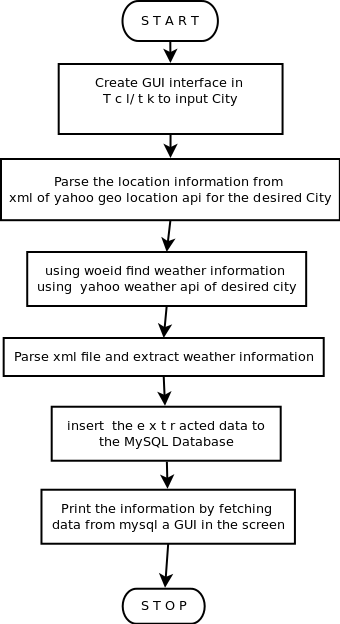
\includegraphics[width=13 cm,height=12 cm]{./flowchart.png}
 % flowchart.png: 239x684 pixel, 72dpi, 8.43x24.13 cm, bb=0 0 239 684
\end{center}


\begin{center}
\chapter{\textcolor{blue}{\underline {EXECUTION INSTRUCTIONS}}}
\end{center}
\begin{enumerate}
 \item For program following instructions are used.
 \begin{enumerate}
  \item chmod 777 wea.tcl
  \item wish wea.tcl
 \end{enumerate}

\end{enumerate}
Input the  name of the City.\\
Repeat the above instructions for different input City name.
\begin{center}
\chapter{\textcolor{blue}{\underline {RESULTS AND CONCLUSIONS}}}\end{center}
\noindent For the given set of city the program exactly displays the weather information of the City.\\
\begin{center}
 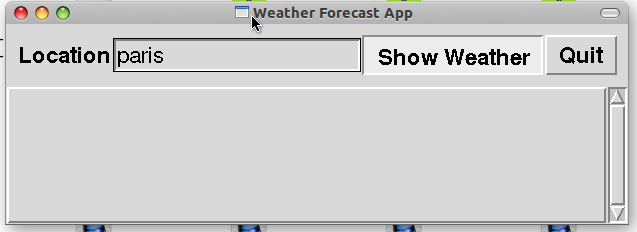
\includegraphics[width=13 cm,height=8 cm]{./Screenshot-1.png}
 
\end{center}
\begin{center}
 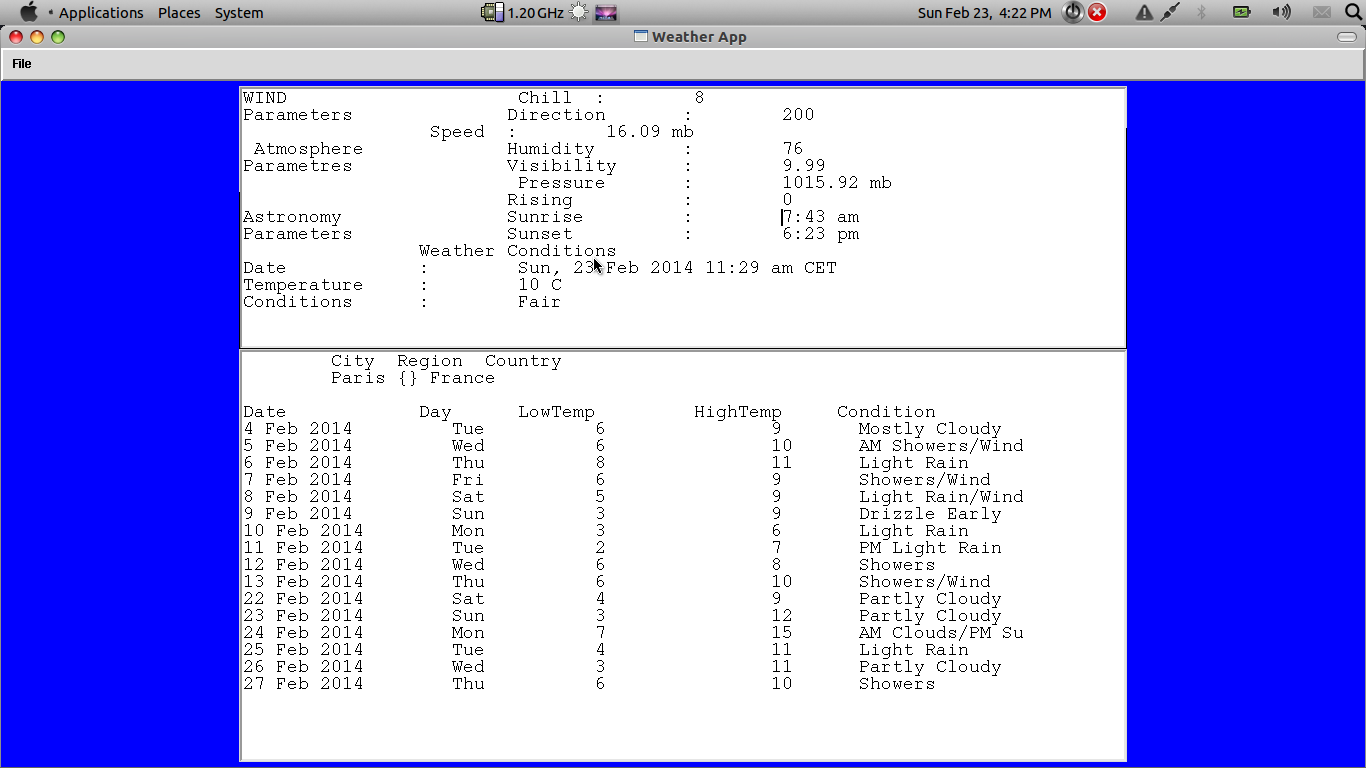
\includegraphics[width=17 cm,height=20 cm]{./Screenshot.png}

\end{center}
\end{document}  